\section{Design}
In this section we designed the system architecture, and created various diagrams to explain how the different parts of the system work.


\subsection{Server-side}
The diagram shown on \ref{fig:serversidestructure} describes the overall structure of the server-side of the system. The server-side consists of both the Web-API and the control panel. These has been combined since they both interact with the same database and both has the same model. 

\begin{figure}[H]
    \centering
    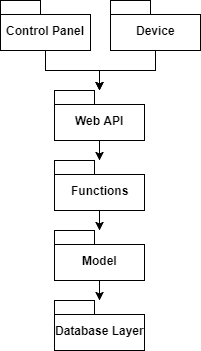
\includegraphics{Figures/serverSide.png}
    \caption{The structure of the server-side part of the system}
    \label{fig:serversidestructure}
\end{figure}

The function-layer is split into two parts, one for the control-panel and one for the API. This is done to isolate the functionality, such that each component only has access to their needed functionality. The shared model layer is described on \ref{fig:serversidemodel}.

\begin{figure}[H]
    \centering 
    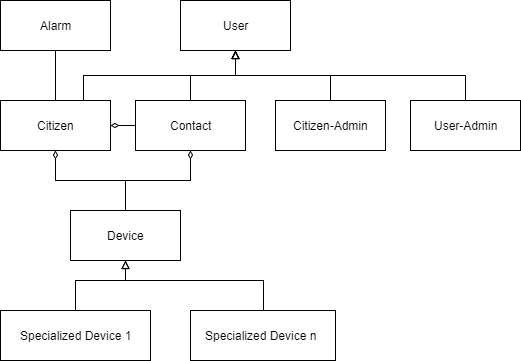
\includegraphics[width=0.9\textwidth]{Figures/serverSidemodel.png}
    \caption{The serverside model}
    \label{fig:serversidemodel}
\end{figure}

% The class-diagram on \ref{fig:serversidemodel} describes the model-layer, and the relations between the different parts of the model-layer.

\subsection{Web-API}
When designing our Web-API, we need a way to interact with it. Here we will look at different ways to interact with a server or service through the use of a Web-API.

\subsubsection{REST}
\todo{source pdf}
REST is based on the HTML protocol, and a REST system allows a client to communicate by using HTTP messages.
The four common message types used in REST are:
\begin{itemize}
\item[GET] Gets a representation of a resource. The use of GET should never have side effects, and multiple calls to get should always give the same result.
\item[DELETE] Deletes a resource. Trying to delete a resource that doesn't exist usually results in an error response, such as 404. DELETE is also idempotent, so sending it multiple times does not cause any damage to the rest of the system, should it be sent twice.
\item[POST] Creates a new resource. Unlike DELETE, POST is not idempotent, so sending the same request twice will create the resource twice. 
The standard also allows POST to be overloaded. POST can do any change: DELETE, PUT, PATCH. When overloading POST, there are no protocol semantics it has to follow.
\item[PUT] Updates\todo{replace?} an existing resource. PUT is also idempotent, as sending the same PUT message multiple times will just update the resource to what it already is. Put can also work as POST for when the resource does not exist.
\end{itemize}

Another HTTP message is PATCH, which works as a partial put, where only some parts of a resource are updated.

REST also have six constrains that have to be fulfilled for the Web-API to be RETSful.

\paragraph{Uniform Interface} 
\paragraph{Stateless} A REST implementation is stateless if the server has no knowledge of the state of the client. All relevant data for the state of the client has to be sent to the server at each call, and nothing is kept between calls.
\paragraph{Cacheable} 
\paragraph{Client-Server} 
\paragraph{Layered SYstem} 
\paragraph{Code on Demand} 

\subsubsection{WSDL}

\subsubsection{SOAP}


\subsection{Control panel}
The diagram shown on \ref{fig:controlpanel} describes the different views in the control panel. The login view is the view shown, when a user must login to the control panel.\\
The admin view, is the view shown to users with administration rights. The view will make the admin able to add new users to the system from the view.\\
The citizen view is for users with citizen-admin rights. The view will show the information on all the citizen the citizen-admin is administrating.

\begin{figure}[H]
    \centering
    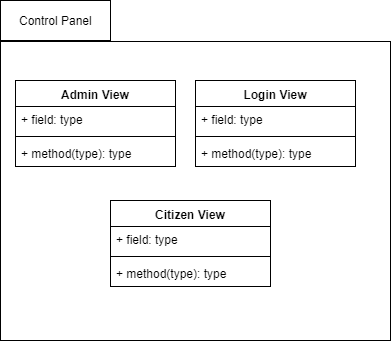
\includegraphics[width=0.5\textwidth]{Figures/ControlPanel.png}
    \caption{The different views included in the control-panel}
    \label{fig:controlpanel}
\end{figure}

\subsection{Smartphone app}

\subsection{Personal assistant}